% !TeX encoding = UTF-8
% !TeX program = xelatex
% !TeX spellcheck = en_US

\documentclass[font=times,fontset=windows,openright]{tyutthesis}
  % 学位 degree:
  %   doctor | master | postdoc
  % 学位类型 degree-type:
  %   academic(默认)| professional
  % 语言 language
  %   chinese(默认)| english
  % 字体库 fontset
  %   windows | mac | fandol | ubuntu
  % 研究生院建议终版使用 Windows 平台的字体编译

% 论文基本配置,加载宏包等全局配置
% !TeX root = ./example.tex

% 论文基本信息配置

\thusetup{
  %******************************
  % 注意:
  %   1. 配置里面不要出现空行
  %   2. 不需要的配置信息可以删除
  %   3. 建议先阅读文档中所有关于选项的说明
  %******************************
  %
  % 输出格式
  %   选择打印版(print)或用于提交的电子版(electronic),前者会插入空白页以便直接双面打印
  %
  output = print,
  %
  % 标题
  %   可使用“\\”命令手动控制换行
  %
  title  = {基于\LaTeX 的毕业论文编写\\方法的研究},
  title* = {The Research on writting method\\ of Dissertation Based on \\ \LaTeX },
  %
  %
  % 培养单位
  %   填写所属院系的全名
  %
  department = {信息与计算机学院},
  department* = {College of Information and Computer},
  %
  % 姓名
  author  = {李小明},
  author* = {Xiaoming Li},
  % 学位 
  degree = master,
  % 学位类型
  degree-type = professional,
  %
  % 日期
  %   使用 ISO 格式;默认为当前时间
  %
  % date = {2019-07-07},
  %
  % 密级和年限
  %   秘密, 机密, 绝密
  %
  % secret-level = {秘密},
  % secret-year  = {10},
  %
  % 博士后专有部分 
  %
  % clc                = {xxx}, % 分类号
  % udc                = {UDC},
  % id                 = {编号},
  % discipline-level-1 = {计算机科学与技术},  % 流动站(一级学科)名称
  % discipline-level-2 = {系统结构},          % 专业(二级学科)名称
  % start-date         = {2011-07-01},        % 研究工作起始时间
}

% 载入所需的宏包
\usepackage{subfig}
\DeclareSubrefFormat{parens}{#1\,(#2)} 
\captionsetup[subfloat]{subrefformat=parens} % 修改:引用子图要有括号。

% 修改:太原理工大学:添加算法环境
\usepackage{algorithm}
\usepackage{algorithmicx}
\usepackage{algpseudocode}
\renewcommand{\algorithmicrequire}{\textbf{输入:}}  
\renewcommand{\algorithmicensure}{\textbf{输出:}} 
% 定义算法字体为五号。自己按情况修改。
\makeatletter
\algrenewcommand\ALG@beginalgorithmic{\wuhao}
\makeatother


%\usepackage{setspace} % 与cls文件中的\@floatboxreset冲突
% 定理类环境宏包
\usepackage{amsthm}
% 也可以使用 ntheorem
% \usepackage[amsmath,thmmarks,hyperref]{ntheorem}
\usepackage{mathtools}

\thusetup{
  %
  % 数学字体
  math-style = GB,  % GB | ISO | TeX
  math-font  = xits,  % sitx | xits | libertinus
}

% 可以使用 nomencl 生成符号和缩略语说明
% \usepackage{nomencl}
% \makenomenclature

% 表格加脚注
\usepackage{threeparttable}

% 表格中支持跨行
\usepackage{multirow}

% 固定宽度的表格。
% \usepackage{tabularx}

% 跨页表格
\usepackage{longtable}
% 单元格
\usepackage{makecell}

% 量和单位
\usepackage{siunitx}

% 参考文献使用 BibTeX + natbib 宏包
% 顺序编码制
\usepackage[sort]{natbib}
\bibliographystyle{thuthesis-numeric}
%\bibliographystyle{gbt7714-numerical}
% 著者-出版年制
% \usepackage{natbib}
% \bibliographystyle{thuthesis-author-year}

% 本科生参考文献的著录格式
% \usepackage[sort]{natbib}
% \bibliographystyle{thuthesis-bachelor}

% 参考文献使用 BibLaTeX 宏包
% \usepackage[backend=biber,style=thuthesis-numeric]{biblatex}
% \usepackage[backend=biber,style=thuthesis-author-year]{biblatex}
% \usepackage[backend=biber,style=apa]{biblatex}
% \usepackage[backend=biber,style=mla-new]{biblatex}
% 声明 BibLaTeX 的数据库
% \addbibresource{ref/refs.bib}

% 定义所有的图片文件在 figures 子目录下
\graphicspath{{figures/}}

% 数学命令
\makeatletter
\newcommand\dif{%  % 微分符号
  \mathop{}\!%
  \ifthu@math@style@TeX
    d%
  \else
    \mathrm{d}%
  \fi
}
\makeatother

% hyperref 宏包在最后调用
\usepackage{hyperref}
\usepackage{color}
\usepackage{rotfloat} % 图片横排
\usepackage[export]{adjustbox} % 图片顶端对齐
% 写作时参考文献位置占位
\newcommand*{\needcite}{\color{red}[cite]}


\begin{document}
\covermatter% 新增:封面部分
% 封面
%\maketitle

% !TeX root = ../example.tex

\makeatletter
% 申请学位的学科门类:小二号宋体字,字距延伸0.5bp,所以\CJKglue应该设为1 bp。
% 修改:太原理工大学学科门类:学历:初号楷体,门类:20bp楷体 楷体均加粗,所以此处使用伪粗楷
% 学位名称
\newcommand\tyut@titlepage@degree{%
	\thu@stretch{11.3cm}{\bfseries\chuhao\kaishu%使用模板定义的弹性盒子
		\ifthu@degree@doctor
			博士%
		\else
			\ifthu@degree@master
				硕士%
			\fi
		\fi%
		学位论文%
	}%
}%

% 学位类型
%\newcommand\tyut@titlepage@degree@type{%
%	\begingroup
%	\CJKfamily+{} % \CJKfamily+ 对所有字符均有效,详见xeCJK
%%\xiaoer
%%	\def\CJKglue{\hskip 1bp}%
%	\bfseries\kaishu\fontsize{20bp}{31.2bp}\selectfont
%	\ifthu@degree@master
%	\ifthu@degree@type@professional
%	(专\ 业\  %
%	\else
%	\ifthu@degree@type@academic
%	(学\ 术\  %
%	\fi
%	\fi
%	学\ 位)
%	\fi
%	\endgroup
%}

\newcommand\tyut@titlepage@degree@type{%
	\centering
	\thu@stretch{4.8cm}{\bfseries\fontsize{20bp}{31.2bp}\selectfont\kaishu%
		\ifthu@degree@master
			\ifthu@degree@type@professional
				(专业%
			\else
				\ifthu@degree@type@academic
					(学术%
				\fi
			\fi%
			学位)%
		\fi%
	}%
}%

% 标题页作者信息表
\newcommand\tyut@titlepage@info@tabular[4]{%
	\def\tyut@info@item##1##2{%
		\thu@pad{#1}{\thu@fixed@box{#2}{##1}}%
		%      \thu@pad{#3}{:}% 修改:太原理工大学要求姓名信息居中,且需要添加下划线,\smash可以得到更接近文字的下划线。
		% 可以选择用\CJKunderline[thickness=<width>]{contents}来调整线宽
		\underline{\smash{\makebox[6cm][c]{##2}}} \\ 
	}%
	\begin{tabular}{l}%
		\renewcommand\arraystretch{1}%
		#4%
	\end{tabular}%
}

% 具体列表:可以自己添加
\newcommand\tyut@titlepage@info{%
	\tyut@titlepage@info@tabular{2.8cm}{2.82cm}{0cm}{%
		\tyut@info@item{姓名:}{\thu@author}%
		\tyut@info@item{学号:}{2000123456}%
		\tyut@info@item{培养单位:}{\thu@department}%
		\tyut@info@item{专业领域:}{计算机技术}%
		\tyut@info@item{研究方向:}{硕士论文}%
		\tyut@info@item{导师姓名:}{XXX \quad 讲师}%
		\tyut@info@item{企业导师:}{XXX \quad 教授}%
	}\par
}

% 论文成文打印的日期,用三号宋体汉字,字距延伸0.5bp,所以\CJKglue应该设为1 bp
\newcommand\tyut@titlepage@date{%
	\begingroup
	\kaishu\sanhao
	% 修改:太原理工大学要求三号楷体,阿拉伯数字日期,不做字距延伸
	论文提交日期:\thu@format@date{\thu@date@zh@digit@short}{\thu@date}\par
	\endgroup
}

% 英文封面格式
\newcommand\tyut@titlepage@en@title{%题目
	\begingroup
	\bfseries\xiaoer\selectfont
	\thu@title@en\par
	\endgroup
}
\newcommand\tyut@thesis@name@en{%
	\ifthu@degree@master
	Thesis%
	\else
	Dissertation%
	\fi
}

\newcommand\tyut@titlepage@en@date{%日期 修改:太原理工大学要求newtimes字体四号行距1.5
	\begingroup
	\sihao[27.4bp]
	\thu@format@date{\thu@date@en@short}{\thu@date}\par
	\endgroup
}

% 中文封面
\newcommand\tyut@titlepage@cn{
	\newgeometry{
		top     = 2.54cm,
		bottom  = 2.54cm,
		hmargin = 3.18cm,
	}%
	
	\thispagestyle{empty}%
	\thusetup{language = chinese}%
	\begingroup % 修改:太原理工大学,分类号,学校代码,密级在顶部左右两侧,小四字体
	{\kaishu\xiaosi%
		\setlength{\parindent}{0em}
		分类号:{\fontsize{11pt}{13.2pt}\thu@clc}\hfill
		学校代码:\makebox[1.35cm][l]{{\fontsize{11pt}{13.2pt}10112}{\enspace}}\par
		\hfill 密\quad\enspace 级:\makebox[1.35cm][l]{\thu@titlepage@secret} \par
	}%
	%    \parbox[t][2cm][t]{\textwidth}{%
		%      \hskip -21.5pt%
		%      \thu@titlepage@secret
		%    }\par
	\centering % logo,学历
	\vskip 34.32pt%
	\parbox{\textwidth}{
		\centering
		
\includegraphics[height=2.62cm,width=10.79cm]{logo.png}
	}
	\vskip 12pt%
	\tyut@titlepage@degree
	\vskip 16pt
	\quad\tyut@titlepage@degree@type
	\vskip 68.64pt%
	%	\vfill
	% 题目
	\begingroup
	\sffamily\fontsize{22bp}{46.8bp}\selectfont
	\bfseries\kaishu \erhao\thu@title\par
	\endgroup
	\ifthu@main@language@english
	\vskip 5.4pt%
	\begingroup
	\sffamily\bfseries\fontsize{20bp}{31.2bp}\selectfont
	\thu@title@en\par
	\endgroup
	\vskip -9.2pt%
	\fi
	%    \vskip 34.1pt%
	\vfill
	\parbox[t][7.25cm][t]{\textwidth}{% 
		% 修改:太原理工大学作者及导师信息部分使用三号楷体
		% 行距需要手动调整
		\centering
		\kaishu\sanhao[30.5bp]\selectfont % 此处为字体字号
		\tyut@titlepage@info % 此处为作者导师信息
	}\par
	\vskip 80bp
	\parbox[t][0.6cm][t]{\textwidth}{\centering\tyut@titlepage@date}\par
	\vskip 16bp
	\endgroup
	\clearpage
	\restoregeometry
	\thu@reset@main@language
}
% 英文封面
\newcommand\tyut@titlepage@en{
	\newgeometry{
		top     = 2.54cm,
		bottom  = 2.54cm,
		hmargin = 3.18cm,
	}%
	\thispagestyle{empty}%
	\thusetup{language = english}%
	\begingroup%
	\centering%
	\null\vskip 8pt%
	\begingroup
	\fontsize{15bp}{31.5bp}\selectfont A Dissertation Submitted to
	\\
	Taiyuan University of Technology
	\\
	In partial fulfillment of the requirement
	\\
	For the degree of %
	\ifthu@degree@doctor
	Doctor
	\else
	\ifthu@degree@master
	Master
	\fi
	\fi%
	\\
	\endgroup
	\vskip 4.6cm%
	\tyut@titlepage@en@title
	\vskip 49.92bp%
	\sihao By\par%
	\sihao[27.3bp]\thu@author@en\par%
	\vfill
	\sihao[27.3bp]\thu@department@en\\
	\vskip 3pt%
	\tyut@titlepage@en@date
	\vskip 22.5pt%
	\endgroup
	\thu@reset@main@language
	\clearpage
	\restoregeometry
}
\makeatother

\begin{titlepage}
	\makeatletter
	\cleardoublepage
	\thu@pdfbookmark{-1}{\thu@title}%
	\tyut@titlepage@cn
	\cleardoublepage
	\tyut@titlepage@en
	\cleardoublepage
	\makeatother
\end{titlepage}

% 学位论文指导小组、公开评阅人和答辩委员会名单
%% !TeX root = ../example.tex
\begingroup
\thispagestyle{empty}%
\null\par
\vskip 4bp%
\begin{center}
	\sffamily\sanhao 学位论文答辩信息表
\end{center}%
\vskip 18bp%
\fontsize{14bp}{35.5bp}\selectfont
%\renewcommand{\arraystretch}{1.7}
\newlength{\lw}
\setlength{\lw}{2\tabcolsep+\arrayrulewidth}
\centering	
\makeatletter
\begin{tabular}{|>{\centering\arraybackslash}m{3.5cm - \lw}|>{\centering\arraybackslash}m{4.75cm- \lw}|>{\centering\arraybackslash}m{3.25cm- \lw}|>{\centering\arraybackslash}m{4.25cm- \lw}|}
	\hline
	{\centering 论文题目}  & \multicolumn{3}{l|}{ }                       \\
	\ifthu@degree@doctor
		\@empty
	\else
		\ifthu@degree@type@professional%
			\hline
			\makecell[c]{论文类型 \\ (在{[\quad]}内打 \\ “√”)} 
			&\multicolumn{3}{@{}c@{}|}{
				\raisebox{-1em}{\makecell[c]{
						{[\quad]}产品研发\qquad {[\quad]}工程设计\qquad {[\quad]}应用研究\\ 
						{[\quad]}工程/项目管理\qquad {[\quad]}调研报告\qquad {[\quad]}基础研究 
				}}
			}\\
		\fi
	\fi%

	\hline
	{答辩日期}  & { }     & 答辩秘书      &   { }  \\
	\hline
	\multicolumn{4}{|@{}c@{}|}{学位论文答辩委员会成员}  \\
	\hline
	\multicolumn{4}{|@{}c@{}|}{%	
		\begin{tabular}[c]{>{\centering\arraybackslash}m{2.75cm- \lw}|>{\centering\arraybackslash}m{3cm- \lw}|>{\centering\arraybackslash}m{5.75cm- \lw}|>{\centering\arraybackslash}m{4.25cm- \lw}}
			姓名           & 职称 & 工作单位 & 备注  \\
			\hline
			&     &      & 主席  \\
			\hline
			&    &       &     \\
			\hline
			&     &       &    \\
			\hline
			\ifthu@degree@doctor
				&    &       &     \\
				\hline
				&     &       &    \\
				\hline
			\fi
		\end{tabular} 
	} \\
\end{tabular}
\makeatother
\endgroup

% !TeX root = ../document.tex
\begingroup
\thispagestyle{empty}%
\fontsize{14bp}{20pt}\selectfont
\null\par
\vskip 4bp%
\begin{center}
	\sffamily\sanhao 学位论文原创性声明
\end{center}%
\vskip 18bp%

本人郑重声明:所呈交的学位论文,是本人在导师的指导下,独立进
行研究所取得的成果。除文中已经注明引用的内容外,本论文不包含其他
个人或集体已发表或撰写过的科研成果。对本文的研究做出贡献的个人和
集体,均已在文中以明确方式标明。本声明的法律责任由本人承担。\par
\vskip 40pt%
\noindent 论文作者签名:\hfill              签字日期:\hspace{2em} 年\hspace{1em} 月 \hspace{1em} 日\hspace{2em}\null\par

\vskip 4.2cm%

\vskip 4bp%
\begin{center}
	\sffamily\sanhao 学位论文版权使用授权书
\end{center}%
\vskip 18bp%

本学位论文作者和指导教师完全了解太原理工大学有关保留、使用学位论文的规定:学校有权保留并向国家有关部门或机构送交学位论文的复印件和电子版;允许本学位论文被查阅和借阅;学校可以将本学位论文的全部或部分内容编入有关数据库进行检索,可以采用影印、缩印或其他复制手段保存和汇编本学位论文。\par
\vskip 20pt%
本学位论文属于:保密\hspace{.5em} \raisebox{.15ex}{$\square$} \hspace{2em} 在\underline{\smash{\makebox[3em][l]{\null}}}年解密后适用本授权书\par
\vskip 20pt%
\hspace{3.58cm} 不保密 \raisebox{.15ex}{$\square$}
\vskip 40pt%
\noindent\makebox[8.5cm][l]{论文作者签名:} 导师签名:\par
\vskip 20pt%
\noindent\makebox[8.5cm][l]{签字日期:\hspace{2em} 年\hspace{1em} 月 \hspace{1em} 日} 签字日期:\hspace{2em} 年\hspace{1em} 月 \hspace{1em} 日\par
\endgroup

\cleardoublepage
% !TeX root = ../example.tex
\begingroup
\thispagestyle{empty}%
\null\par
\vskip 4bp%
\begin{center}
	\sffamily\sanhao 学位论文答辩信息表
\end{center}%
\vskip 18bp%
\fontsize{14bp}{35.5bp}\selectfont
%\renewcommand{\arraystretch}{1.7}
\newlength{\lw}
\setlength{\lw}{2\tabcolsep+\arrayrulewidth}
\centering	
\makeatletter
\begin{tabular}{|>{\centering\arraybackslash}m{3.5cm - \lw}|>{\centering\arraybackslash}m{4.75cm- \lw}|>{\centering\arraybackslash}m{3.25cm- \lw}|>{\centering\arraybackslash}m{4.25cm- \lw}|}
	\hline
	{\centering 论文题目}  & \multicolumn{3}{l|}{ }                       \\
	\ifthu@degree@doctor
		\@empty
	\else
		\ifthu@degree@type@professional%
			\hline
			\makecell[c]{论文类型 \\ (在{[\quad]}内打 \\ “√”)} 
			&\multicolumn{3}{@{}c@{}|}{
				\raisebox{-1em}{\makecell[c]{
						{[\quad]}产品研发\qquad {[\quad]}工程设计\qquad {[\quad]}应用研究\\ 
						{[\quad]}工程/项目管理\qquad {[\quad]}调研报告\qquad {[\quad]}基础研究 
				}}
			}\\
		\fi
	\fi%

	\hline
	{答辩日期}  & { }     & 答辩秘书      &   { }  \\
	\hline
	\multicolumn{4}{|@{}c@{}|}{学位论文答辩委员会成员}  \\
	\hline
	\multicolumn{4}{|@{}c@{}|}{%	
		\begin{tabular}[c]{>{\centering\arraybackslash}m{2.75cm- \lw}|>{\centering\arraybackslash}m{3cm- \lw}|>{\centering\arraybackslash}m{5.75cm- \lw}|>{\centering\arraybackslash}m{4.25cm- \lw}}
			姓名           & 职称 & 工作单位 & 备注  \\
			\hline
			&     &      & 主席  \\
			\hline
			&    &       &     \\
			\hline
			&     &       &    \\
			\hline
			\ifthu@degree@doctor
				&    &       &     \\
				\hline
				&     &       &    \\
				\hline
			\fi
		\end{tabular} 
	} \\
\end{tabular}
\makeatother
\endgroup

\cleardoublepage
% 使用授权的说明
%\copyrightpage
% 将签字扫描后授权文件 scan-copyright.pdf 替换原始页面
% 声明和授权
% \copyrightpage[file=scan-copyright.pdf]

% 学位论文答辩信息表
%\includepdf

\frontmatter
% !TeX root = ../example.tex

% 中英文摘要和关键字

\begin{abstract}
  摘要是一篇具有独立性和完整性的短文,应概况而扼要地反映出论文的主要内容。
  摘要应对论文所研究的问题及其研究目的进行描述,对研究方法和过程进行简单介绍,对研究成果和所得结论进行概括。
  摘要应具有独立性和自明性,其内容应包含与论文全文同等量的主要信息。
  使读者即使不阅读全文,通过摘要就能了解论文的总体内容和主要成果。
  摘要包括研究目的、方法、结果和结论,要突出论文的创造性成果。摘要中不可出现参考文献、图、表、化学结构式、非公知公用的符号和术语。
  
  论文摘要的书写应力求精确、简明。
  切忌写成对论文书写内容进行提要的形式,尤其要避免“第 1 章……;第 2 章……;……”这种或类似的陈述方式。
  
  英文摘要与中文摘要内容应一致。硕士学位论文摘要不少于 500 字,博士学位论文摘要不少于 1000 字。
  
  关键词是为了便于文献索引和检索,从论文中选取出来用以表示全文主题内容信息的术语。
  关键词一般选 5\textasciitilde8 个专业术语,中、英文关键词须对应。

  % 关键词用“英文逗号”分隔,输出时会自动处理为正确的分隔符
  \thusetup{
    keywords = {关键词 1, 关键词 2, 关键词 3, 关键词 4, 关键词 5},
  }
\end{abstract}

\cleardoublepage
\begin{abstract*}
  An abstract of a dissertation is a summary and extraction of research work and contributions.
  Included in an abstract should be description of research topic and research objective, brief introduction to methodology and research process, and summarization of conclusion and contributions of the research.
  An abstract should be characterized by independence and clarity and carry identical information with the dissertation.
  It should be such that the general idea and major contributions of the dissertation are conveyed without reading the dissertation.

  An abstract should be concise and to the point.
  It is a misunderstanding to make an abstract an outline of the dissertation and words “the first chapter”, “the second chapter” and the like should be avoided in the abstract.

  Keywords are terms used in a dissertation for indexing, reflecting core information of the dissertation.
  An abstract may contain a maximum of 5 keywords, with semi-colons used in between to separate one another.

  % Use comma as seperator when inputting
  \thusetup{
    keywords* = {keyword 1, keyword 2, keyword 3, keyword 4, keyword 5},
  }
\end{abstract*}


\cleardoublepage
% 目录
\begingroup
\hypersetup{hidelinks} % 目录去掉红框更美观
\tableofcontents

% 插图和附表清单
% 本科生的插图索引和表格索引需要移至正文之后、参考文献前
% \listoffiguresandtables  % 插图和附表清单
\listoffigures           % 插图清单
\listoftables            % 附表清单
\endgroup
% 符号对照表
% !TeX root = ../thuthesis-example.tex

\begin{denotation}[3cm]
  \item[PI] 聚酰亚胺
  \item[MPI] 聚酰亚胺模型化合物,N-苯基邻苯酰亚胺
  \item[PBI] 聚苯并咪唑
  \item[MPBI] 聚苯并咪唑模型化合物,N-苯基苯并咪唑
  \item[PY] 聚吡咙
  \item[PMDA-BDA] 均苯四酸二酐与联苯四胺合成的聚吡咙薄膜
  \item[MPY] 聚吡咙模型化合物
  \item[As-PPT] 聚苯基不对称三嗪
  \item[MAsPPT] 聚苯基不对称三嗪单模型化合物,3,5,6-三苯基-1,2,4-三嗪
  \item[DMAsPPT] 聚苯基不对称三嗪双模型化合物(水解实验模型化合物)
  \item[S-PPT] 聚苯基对称三嗪
  \item[MSPPT] 聚苯基对称三嗪模型化合物,2,4,6-三苯基-1,3,5-三嗪
  \item[PPQ] 聚苯基喹噁啉
  \item[MPPQ] 聚苯基喹噁啉模型化合物,3,4-二苯基苯并二嗪
  \item[HMPI] 聚酰亚胺模型化合物的质子化产物
  \item[HMPY] 聚吡咙模型化合物的质子化产物
  \item[HMPBI] 聚苯并咪唑模型化合物的质子化产物
  \item[HMAsPPT] 聚苯基不对称三嗪模型化合物的质子化产物
  \item[HMSPPT] 聚苯基对称三嗪模型化合物的质子化产物
  \item[HMPPQ] 聚苯基喹噁啉模型化合物的质子化产物
  \item[PDT] 热分解温度
  \item[HPLC] 高效液相色谱(High Performance Liquid Chromatography)
  \item[HPCE] 高效毛细管电泳色谱(High Performance Capillary lectrophoresis)
  \item[LC-MS] 液相色谱-质谱联用(Liquid chromatography-Mass Spectrum)
  \item[TIC] 总离子浓度(Total Ion Content)
  \item[\textit{ab initio}] 基于第一原理的量子化学计算方法,常称从头算法
  \item[DFT] 密度泛函理论(Density Functional Theory)
  \item[$E_a$] 化学反应的活化能(Activation Energy)
  \item[ZPE] 零点振动能(Zero Vibration Energy)
  \item[PES] 势能面(Potential Energy Surface)
  \item[TS] 过渡态(Transition State)
  \item[TST] 过渡态理论(Transition State Theory)
  \item[$\increment G^\neq$] 活化自由能(Activation Free Energy)
  \item[$\kappa$] 传输系数(Transmission Coefficient)
  \item[IRC] 内禀反应坐标(Intrinsic Reaction Coordinates)
  \item[$\nu_i$] 虚频(Imaginary Frequency)
  \item[ONIOM] 分层算法(Our own N-layered Integrated molecular Orbital and molecular Mechanics)
  \item[SCF] 自洽场(Self-Consistent Field)
  \item[SCRF] 自洽反应场(Self-Consistent Reaction Field)
\end{denotation}



% 也可以使用 nomencl 宏包,需要在导言区
% \usepackage{nomencl}
% \makenomenclature

% 在这里输出符号说明
% \printnomenclature[3cm]

% 在正文中的任意为都可以标题
% \nomenclature{PI}{聚酰亚胺}
% \nomenclature{MPI}{聚酰亚胺模型化合物,N-苯基邻苯酰亚胺}
% \nomenclature{PBI}{聚苯并咪唑}
% \nomenclature{MPBI}{聚苯并咪唑模型化合物,N-苯基苯并咪唑}
% \nomenclature{PY}{聚吡咙}
% \nomenclature{PMDA-BDA}{均苯四酸二酐与联苯四胺合成的聚吡咙薄膜}
% \nomenclature{MPY}{聚吡咙模型化合物}
% \nomenclature{As-PPT}{聚苯基不对称三嗪}
% \nomenclature{MAsPPT}{聚苯基不对称三嗪单模型化合物,3,5,6-三苯基-1,2,4-三嗪}
% \nomenclature{DMAsPPT}{聚苯基不对称三嗪双模型化合物(水解实验模型化合物)}
% \nomenclature{S-PPT}{聚苯基对称三嗪}
% \nomenclature{MSPPT}{聚苯基对称三嗪模型化合物,2,4,6-三苯基-1,3,5-三嗪}
% \nomenclature{PPQ}{聚苯基喹噁啉}
% \nomenclature{MPPQ}{聚苯基喹噁啉模型化合物,3,4-二苯基苯并二嗪}
% \nomenclature{HMPI}{聚酰亚胺模型化合物的质子化产物}
% \nomenclature{HMPY}{聚吡咙模型化合物的质子化产物}
% \nomenclature{HMPBI}{聚苯并咪唑模型化合物的质子化产物}
% \nomenclature{HMAsPPT}{聚苯基不对称三嗪模型化合物的质子化产物}
% \nomenclature{HMSPPT}{聚苯基对称三嗪模型化合物的质子化产物}
% \nomenclature{HMPPQ}{聚苯基喹噁啉模型化合物的质子化产物}
% \nomenclature{PDT}{热分解温度}
% \nomenclature{HPLC}{高效液相色谱(High Performance Liquid Chromatography)}
% \nomenclature{HPCE}{高效毛细管电泳色谱(High Performance Capillary lectrophoresis)}
% \nomenclature{LC-MS}{液相色谱-质谱联用(Liquid chromatography-Mass Spectrum)}
% \nomenclature{TIC}{总离子浓度(Total Ion Content)}
% \nomenclature{\textit{ab initio}}{基于第一原理的量子化学计算方法,常称从头算法}
% \nomenclature{DFT}{密度泛函理论(Density Functional Theory)}
% \nomenclature{$E_a$}{化学反应的活化能(Activation Energy)}
% \nomenclature{ZPE}{零点振动能(Zero Vibration Energy)}
% \nomenclature{PES}{势能面(Potential Energy Surface)}
% \nomenclature{TS}{过渡态(Transition State)}
% \nomenclature{TST}{过渡态理论(Transition State Theory)}
% \nomenclature{$\increment G^\neq$}{活化自由能(Activation Free Energy)}
% \nomenclature{$\kappa$}{传输系数(Transmission Coefficient)}
% \nomenclature{IRC}{内禀反应坐标(Intrinsic Reaction Coordinates)}
% \nomenclature{$\nu_i$}{虚频(Imaginary Frequency)}
% \nomenclature{ONIOM}{分层算法(Our own N-layered Integrated molecular Orbital and molecular Mechanics)}
% \nomenclature{SCF}{自洽场(Self-Consistent Field)}
% \nomenclature{SCRF}{自洽反应场(Self-Consistent Reaction Field)}


\mainmatter
% 正文部分
% !TeX root = ../example.tex

\chapter{论文主要部分的写法}

研究生学位论文撰写,除表达形式上需要符合一定的格式要求外,内容方面上也要遵循一些共性原则。

通常研究生学位论文只能有一个主题(不能是几块工作拼凑在一起),该主题应针对某学科领域中的一个具体问题展开深入、系统的研究,并得出有价值的研究结论。
学位论文的研究主题切忌过大,例如,“中国国有企业改制问题研究”这样的研究主题过大,因为“国企改制”涉及的问题范围太广,很难在一本研究生学位论文中完全研究透彻。



\section{论文的语言及表述}

除国际研究生外,学位论文一律须用汉语书写。
学位论文应当用规范汉字进行撰写,除古汉语研究中涉及的古文字和参考文献中引用的外文文献之外,均采用简体汉字撰写。

国际研究生一般应以中文或英文书写学位论文,格式要求同上。
论文须用中文封面。

研究生学位论文是学术作品,因此其表述要严谨简明,重点突出,专业常识应简写或不写,做到立论正确、数据可靠、说明透彻、推理严谨、文字凝练、层次分明,避免使用文学性质的或带感情色彩的非学术性语言。

论文中如出现一个非通用性的新名词、新术语或新概念,需随即解释清楚。

\subsection{子节的格式}

论文一般使用二级节标题,根据情况使用三级节标题。


\section{论文题目的写法}

论文题目应简明扼要地反映论文工作的主要内容,力求精炼、准确,切忌笼统。
论文题目是对研究对象的准确、具体描述,一般要在一定程度上体现研究结论,因此,论文题目不仅应告诉读者这本论文研究了什么问题,更要告诉读者这个研究得出的结论。
例如:“在事实与虚构之间:梅乐、卡彭特、沃尔夫的新闻观”就比“三个美国作家的新闻观研究”更专业、更准确。



\section{摘要的写法}

论文摘要是对论文研究内容的高度概括,应具有独立性和自含性,即应是 一篇简短但意义完整的文章。
通过阅读论文摘要,读者应该能够对论文的研究 方法及结论有一个整体性的了解,因此摘要的写法应力求精确简明。
论文摘要 应包括对问题及研究目的的描述、对使用的方法和研究过程进行的简要介绍、 对研究结论的高度凝练等,重点是结果和结论。

论文摘要切忌写成全文的提纲,尤其要避免“第 1 章……;第 2 章……;……”这样的陈述方式。



\section{引言的写法}

一篇学位论文的引言大致包含如下几个部分:
1、问题的提出;
2、选题背 景及意义;
3、文献综述;
4、研究方法;
5、论文结构安排。
\begin{itemize}
  \item 问题的提出:要清晰地阐述所要研究的问题“是什么”。
    \footnote{选题时切记要有“问题意识”,不要选不是问题的问题来研究。}
  \item 选题背景及意义:论述清楚为什么选择这个题目来研究,即阐述该研究对学科发展的贡献、对国计民生的理论与现实意义等。
  \item 文献综述:对本研究主题范围内的文献进行详尽的综合述评,“述”的同时一定要有“评”,指出现有研究状态,仍存在哪些尚待解决的问题,讲出自己的研究有哪些探索性内容。
  \item 研究方法:讲清论文所使用的学术研究方法。
  \item 论文结构安排:介绍本论文的写作结构安排。
\end{itemize}



\section{正文的写法}

本部分是论文作者的研究内容,不能将他人研究成果不加区分地掺和进来。
已经在引言的文献综述部分讲过的内容,这里不需要再重复。
各章之间要存在有机联系,符合逻辑顺序。

本部分是论文作者的研究内容,是论文的核心。由于涉及不同的学科,存在
差异,不作统一的规定。论文应结构合理,层次清楚,重点突出。各章之间互相
关联,符合逻辑顺序。其中,工程硕士论文可以是产品研发、工程设计、应用研
究、工程/项目管理、调研报告,也可以是研究论文,具体撰写要求参考《太原
理工大学工程类专业硕士学位论文基本要求》。

正文中标号按如下编号格式顺序排列:先(1)、(2)、(3),再 1)、2)、3),后①、②、③。

\section{结论的写法}

结论是对论文主要研究结果、论点的提炼与概括,应精炼、准确、完整,使读者看后能全面了解论文的意义、目的和工作内容。
结论单独作为最后一章,是整个论文最终和总体的结论,不是正文中各章小结的简单重复。应明确指出本研究的创新点,对其应用前景和社会经济价值等加
以预测和评价,指出今后进一步在本研究方向进行研究工作的展望与设想。

同时,要严格区分自己取得的成果与指导教师及他人的学术成果。

在评价自己的研究工作成果时,要实事求是,除非有足够的证据表明自己的研究是“首次”、“领先”、“填补空白”的,否则应避免使用这些或类似词语。

% !TeX root = ../example.tex

\chapter{图表示例}

\section{插图}

图片通常在 \env{figure} 环境中使用 \cs{includegraphics} 插入,如图~\ref{fig:example} 的源代码。
建议矢量图片使用 PDF 格式,比如数据可视化的绘图;
照片应使用 JPG 格式;
其他的栅格图应使用无损的 PNG 格式。
注意,LaTeX 不支持 TIFF 格式;EPS 格式已经过时。

\begin{figure}
  \centering
  
\includegraphics[width=0.6\linewidth]{example-image-a.pdf}
  \bicaption{示例图片}{Example figure}
  \label{fig:example}
\end{figure}

图包括曲线图、构造图、示意图、框图、流程图、记录图、照片等。
图应具有自明性,一般随文编排,先文字后见图。
图中各部分说明应采用中文(引用的外文图除外)或数字符号,各项文字说明置于图下图题之上。


图序与图题:图序即图的编号,由“图”和阿拉伯数字组成,较多时可按章依序编号,如图 1-1、图 1-2。图题即图的名称,置于图序之后,图序和图题间
空 1 个字符,中英文对照,居中置于图的下方,中文在上。该模板中使用 \pkg{bicaption} 宏包实现双语图题。如有分图时,分图号用(a)、(b)表示,分图题置于分图之下或图题之下。如放在图题之下,多个分图题之间用“;”隔开,\emph{末尾不加句点}。
引用文献中的图时,除在正文中标注参考文献序号以外,还必须在中、英文图题的右上角标注参考文献序号。
推荐使用 \pkg{subfig} 宏包来处理, 比如图~\subref*{fig:subfig-a} 和图~\subref*{fig:subfig-b}。

若图或表中有附注,采用英文小写字母顺序编号,附注写在图或表的下方。
% LaTeX 传统上一般将附注的内容同图表的标题写在一起,形成很长的一段文字。

如论文中图表较多,可以分别列出清单置于目录页之后。图的清单应有序号、图题和页码。表的清单应有序号、表题和页码。

\begin{figure}
  \centering
  \subfloat[分图 A\label{fig:subfig-a}]
    {
\includegraphics[width=0.4\linewidth]{example-image-a.pdf}}
  \subfloat[分图 B\label{fig:subfig-b}]
    {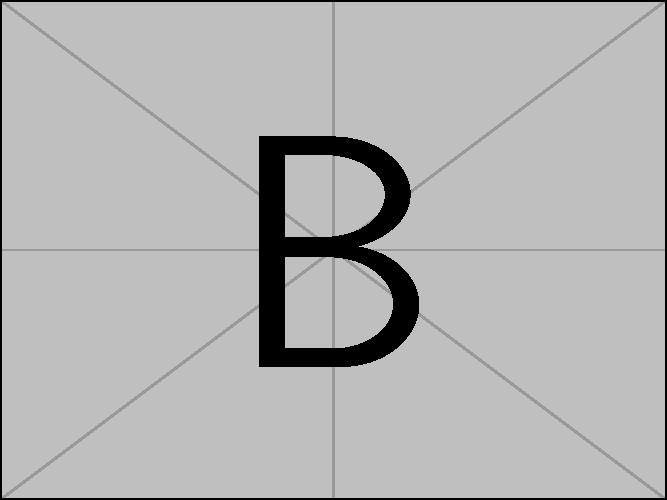
\includegraphics[width=0.4\linewidth]{example-image-b.pdf}}
  \bicaption[多个分图的示例]{% 总图题写在方括号内,其显示在插图列表中
  	多个分图的示例:(a) 左图;(b) 右图
  }{
  	Multiple subfigure example:
  	(a) figure on the left; (b)	figure on the right
  }
  \label{fig:multi-image}
\end{figure}



\section{表格}

表应具有自明性。为使表格简洁易读,尽可能采用三线表,如表~\ref{tab:three-line}。
三条线可以使用 \pkg{booktabs} 宏包提供的命令生成。

\begin{table}[!htb]
  \centering
  \bicaption{三线表示例}{Table with three rules}
  \begin{tabular}{ll}
    \toprule
    文件名          & 描述                         \\
    \midrule
    thuthesis.dtx   & 模板的源文件,包括文档和注释 \\
    thuthesis.cls   & 模板文件                     \\
    thuthesis-*.bst & BibTeX 参考文献表样式文件    \\
    thuthesis-*.bbx & BibLaTeX 参考文献表样式文件  \\
    thuthesis-*.cbx & BibLaTeX 引用样式文件        \\
    \bottomrule
  \end{tabular}
  \label{tab:three-line}
\end{table}

表格如果有附注,尤其是需要在表格中进行标注时,可以使用 \pkg{threeparttable} 宏包。

\begin{table}[!htb]
  \centering
  \begin{threeparttable}[c]
    \bicaption{带附注的表格示例}{Table example with notes}
    \label{tab:three-part-table}
    \begin{tabular}{ll}
      \toprule
      文件名                 & 描述                         \\
      \midrule
      thuthesis.dtx\tnote{a} & 模板的源文件,包括文档和注释 \\
      thuthesis.cls\tnote{b} & 模板文件                     \\
      thuthesis-*.bst        & BibTeX 参考文献表样式文件    \\
      thuthesis-*.bbx        & BibLaTeX 参考文献表样式文件  \\
      thuthesis-*.cbx        & BibLaTeX 引用样式文件        \\
      \bottomrule
    \end{tabular}
    \begin{tablenotes}
      \item [a] 可以通过 xelatex 编译生成模板的使用说明文档;
        使用 xetex 编译 \file{thuthesis.ins} 时则会从 \file{.dtx} 中去除掉文档和注释,得到精简的 \file{.cls} 文件。
      \item [b] 更新模板时,一定要记得编译生成 \file{.cls} 文件,否则编译论文时载入的依然是旧版的模板。
    \end{tablenotes}
  \end{threeparttable}
\end{table}

如某个表需要转页接排,可以使用 \pkg{longtable} 宏包,需要在随后的各页上重复表的编号。
编号后跟表题(可省略)和“(续)”,置于表上方。续表均应重复表头。

\begin{longtable}{cccc}
	\bicaption{跨页长表格的表题}{Longtable example} \\
	\toprule
	表头 1 & 表头 2 & 表头 3 & 表头 4 \\
	\midrule
	\endfirsthead
	\bicaption[]{跨页长表格的表题(续)}{Longtable example(continue)} \\
	\toprule
	表头 1 & 表头 2 & 表头 3 & 表头 4 \\
	\midrule
	\endhead
	\bottomrule
	\endfoot
	Row 1  & & & \\
	Row 2  & & & \\
	Row 3  & & & \\
	Row 4  & & & \\
	Row 5  & & & \\
	Row 6  & & & \\
	Row 7  & & & \\
	Row 8  & & & \\
	Row 9  & & & \\
	Row 10 & & & \\
	Row 11 & & & \\
	Row 12 & & & \\
	Row 13 & & & \\
	Row 14 & & & \\
	Row 15 & & & \\
	Row 16 & & & \\
	Row 17 & & & \\
	Row 18 & & & \\
	Row 19 & & & \\
	Row 20 & & & \\
	Row 21 & & & \\
	Row 22 & & & \\
	Row 23 & & & \\
	Row 24 & & & \\
	Row 25 & & & \\
	Row 26 & & & \\
	Row 27 & & & \\
	Row 28 & & & \\
	Row 29 & & & \\
	Row 30 & & & \\
	Row 31 & & & \\
	Row 32 & & & \\
	Row 33 & & & \\
	Row 34 & & & \\
	Row 35 & & & \\
	Row 36 & & & \\
	Row 37 & & & \\
	Row 38 & & & \\
	Row 39 & & & \\
	Row 40 & & & \\
	Row 41 & & & \\
	Row 42 & & & \\
	Row 43 & & & \\
	Row 44 & & & \\
	Row 45 & & & \\
	Row 46 & & & \\
	Row 47 & & & \\
	Row 48 & & & \\
	Row 49 & & & \\
	Row 50 & & & \\
\end{longtable}

算法可以使用\pkg{algorithm}、\pkg{algorithmicx}、\pkg{algpseudocode}等宏包实现。欧几里得算法过程如算法~\ref{euclid}所示。
\begin{algorithm}[!htb]
	\caption{欧几里得算法}
	\label{euclid}
	\begin{algorithmic}[1]
		\Require 两个正整数$a$, $b$
		\Ensure 最大公约数
		\Procedure{Euclid}{$a,b$}\Comment{$a$ 和 $b$ 的最大公约数}
		\State $r \gets a \bmod b$
		\While{$r \not= 0$}\Comment{若$r$为0,则直接返回}
		\State $a \gets b$
		\State $b \gets r$
		\State $r \gets a \bmod b$
		\EndWhile\label{euclidendwhile}
		\State \textbf{return} $b$\Comment{最大公约数为$b$}
		\EndProcedure
	\end{algorithmic}
\end{algorithm}
% !TeX root = ../example.tex

\chapter{数学符号和公式}

\section{数学符号}
表达式主要指数字表达式,也包括文字表达式。表达式需另行起排,并用阿拉伯数字分章编号,序号加圆括号,右顶格排。表达式的编号为小四号 Times New
Roman。

中文论文的数学符号默认遵循 GB/T 3102.11—1993《物理科学和技术中使用的数学符号》
\footnote{原 GB 3102.11—1993,自 2017 年 3 月 23 日起,该标准转为推荐性标准。}。
该标准参照采纳 ISO 31-11:1992 \footnote{目前已更新为 ISO 80000-2:2019。},
但是与 \TeX{} 默认的美国数学学会(AMS)的符号习惯有所区别。
具体地来说主要有以下差异:
\begin{enumerate}
  \item 大写希腊字母默认为斜体,如
    \begin{equation*}
      \Gamma \Delta \Theta \Lambda \Xi \Pi \Sigma \Upsilon \Phi \Psi \Omega.
    \end{equation*}
    注意有限增量符号 $\increment$ 固定使用正体,模板提供了 \cs{increment} 命令。
  \item 小于等于号和大于等于号使用倾斜的字形 $\le$、$\ge$。
  \item 积分号使用正体,比如 $\int$、$\oint$。
  \item 行间公式积分号的上下限位于积分号的上下两端,但看起来不美观,因此仍然将上下限统一居右侧,比如
    \begin{equation*}
      \int_a^b f(x) \dif x.
    \end{equation*}
    行内公式为了版面的美观,统一居右侧,如 $\int_a^b f(x) \dif x$ 。
  \item
    偏微分符号 $\partial$ 使用正体。
  \item
    省略号 \cs{dots} 按照中文的习惯固定居中,比如
    \begin{equation*}
      1, 2, \dots, n \quad 1 + 2 + \dots + n.
    \end{equation*}
  \item
    实部 $\Re$ 和虚部 $\Im$ 的字体使用罗马体。
\end{enumerate}

以上数学符号样式的差异可以在模板中统一设置。
另外国标还有一些与 AMS 不同的符号使用习惯,需要用户在写作时进行处理:
\begin{enumerate}
  \item 数学常数和特殊函数名用正体,如
    \begin{equation*}
      \uppi = 3.14\dots; \quad
      \symup{i}^2 = -1; \quad
      \symup{e} = \lim_{n \to \infty} \left( 1 + \frac{1}{n} \right)^n.
    \end{equation*}
  \item 微分号使用正体,比如 $\dif y / \dif x$。
  \item 向量、矩阵和张量用粗斜体(\cs{symbf}),如 $\symbf{x}$、$\symbf{\Sigma}$、$\symbfsf{T}$。
  \item 自然对数用 $\ln x$ 不用 $\log x$。
\end{enumerate}


英文论文的数学符号使用 \TeX{} 默认的样式。
如果有必要,也可以通过设置 \verb|math-style| 选择数学符号样式。

关于量和单位推荐使用
\href{http://mirrors.ctan.org/macros/latex/contrib/siunitx/siunitx.pdf}{\pkg{siunitx}}
宏包,
可以方便地处理希腊字母以及数字与单位之间的空白,
比如:
\SI{6.4e6}{m},
\SI{9}{\micro\meter},
\si{kg.m.s^{-1}},
\SIrange{10}{20}{\degreeCelsius}。



\section{数学公式}

数学公式可以使用 \env{equation} 和 \env{equation*} 环境。
注意数学公式的引用应前后带括号,建议使用 \cs{eqref} 命令,比如式 \eqref{eq:example}。
\begin{equation}
  \frac{1}{2 \uppi \symup{i}} \int_\gamma f = \sum_{k=1}^m n(\gamma; a_k) \mathscr{R}(f; a_k)
  \label{eq:example}
\end{equation}
注意公式编号的引用应含有圆括号,可以使用 \cs{eqref} 命令。

多行公式尽可能在“=”处对齐,推荐使用 \env{align} 环境。
\begin{align}
  a & = b + c + d + e \\
    & = f + g
\end{align}



\section{数学定理}

定理环境的格式可以使用 \pkg{amsthm} 或者 \pkg{ntheorem} 宏包配置。
用户在导言区载入这两者之一后,模板会自动配置 \env{thoerem}、\env{proof} 等环境。

\begin{theorem}[Lindeberg--Lévy 中心极限定理]
  设随机变量 $X_1, X_2, \dots, X_n$ 独立同分布, 且具有期望 $\mu$ 和有限的方差 $\sigma^2 \ne 0$,
  记 $\bar{X}_n = \frac{1}{n} \sum_{i+1}^n X_i$,则
  \begin{equation}
    \lim_{n \to \infty} P \left(\frac{\sqrt{n} \left( \bar{X}_n - \mu \right)}{\sigma} \le z \right) = \Phi(z),
  \end{equation}
  其中 $\Phi(z)$ 是标准正态分布的分布函数。
\end{theorem}
\begin{proof}
  Trivial.
\end{proof}

同时模板还提供了 \env{assumption}、\env{definition}、\env{proposition}、
\env{lemma}、\env{theorem}、\env{axiom}、\env{corollary}、\env{exercise}、
\env{example}、\env{remar}、\env{problem}、\env{conjecture} 这些相关的环境。

% !TeX root = ../example.tex

\chapter{引用文献的标注}
为了反映论文的科学依据和作者尊重他人研究成果的严肃态度以及向读者
提供有关信息的出处,应列出参考文献表。参考文献中列出的一般应限于作者直
接阅读过被引用的、发表在正式出版物上的文献。私人通信和未公开发表的资料,
一般不宜列入参考文献,可紧跟在引用的内容之后注释或标注在当页的下方。
参考文献应置于正文之后,以近几年的文献为主,博士学位论文参考文献不
少于 80 篇,硕士学术学位论文参考文献不少于 40 篇,硕士专业学位论文参考文
献不少于 30 篇。

参考文献表的标注方法可采用顺序编码制,也可采用著者-出版年制。

模板支持 BibTeX 和 BibLaTeX 两种方式处理参考文献。
下文主要介绍 BibTeX 配合 \pkg{natbib} 宏包的主要使用方法。


\section{顺序编码制}

在顺序编码制下,默认的 \cs{cite} 命令同 \cs{citep} 一样,序号置于方括号中,
引文页码会放在括号外。
统一处引用的连续序号会自动用短横线连接。

\thusetup{
  cite-style = super,
}
\begin{tabular}{l@{\quad$\Rightarrow$\quad}l}
  \verb|\cite{zhangkun1994}|               & \cite{zhangkun1994}               \\
  \verb|\citet{zhangkun1994}|              & \citet{zhangkun1994}              \\
  \verb|\citep{zhangkun1994}|              & \citep{zhangkun1994}              \\
  \verb|\cite[42]{zhangkun1994}|           & \cite[42]{zhangkun1994}           \\
  \verb|\cite{zhangkun1994,zhukezhen1973}| & \cite{zhangkun1994,zhukezhen1973} \\
\end{tabular}


也可以取消上标格式,将数字序号作为文字的一部分。
建议全文统一使用相同的格式。

\thusetup{
  cite-style = inline,
}
\begin{tabular}{l@{\quad$\Rightarrow$\quad}l}
  \verb|\cite{zhangkun1994}|               & \cite{zhangkun1994}               \\
  \verb|\citet{zhangkun1994}|              & \citet{zhangkun1994}              \\
  \verb|\citep{zhangkun1994}|              & \citep{zhangkun1994}              \\
  \verb|\cite[42]{zhangkun1994}|           & \cite[42]{zhangkun1994}           \\
  \verb|\cite{zhangkun1994,zhukezhen1973}| & \cite{zhangkun1994,zhukezhen1973} \\
\end{tabular}



\section{著者-出版年制}

著者-出版年制下的 \cs{cite} 跟 \cs{citet} 一样。

\thusetup{
  cite-style = author-year,
}
\begin{tabular}{l@{\quad$\Rightarrow$\quad}l}
  \verb|\cite{zhangkun1994}|                & \cite{zhangkun1994}                \\
  \verb|\citet{zhangkun1994}|               & \citet{zhangkun1994}               \\
  \verb|\citep{zhangkun1994}|               & \citep{zhangkun1994}               \\
  \verb|\cite[42]{zhangkun1994}|            & \cite[42]{zhangkun1994}            \\
  \verb|\citep{zhangkun1994,zhukezhen1973}| & \citep{zhangkun1994,zhukezhen1973} \\
\end{tabular}

\vskip 2ex
\thusetup{
  cite-style = super,
}
注意,引文参考文献的每条都要在正文中标注
\cite{zhangkun1994,zhukezhen1973,dupont1974bone,zhengkaiqing1987,%
  jiangxizhou1980,jianduju1994,merkt1995rotational,mellinger1996laser,%
  bixon1996dynamics,mahui1995,carlson1981two,taylor1983scanning,%
  taylor1981study,shimizu1983laser,atkinson1982experimental,%
  kusch1975perturbations,guangxi1993,huosini1989guwu,wangfuzhi1865songlun,%
  zhaoyaodong1998xinshidai,biaozhunhua2002tushu,chubanzhuanye2004,%
  who1970factors,peebles2001probability,baishunong1998zhiwu,%
  weinstein1974pathogenic,hanjiren1985lun,dizhi1936dizhi,%
  tushuguan1957tushuguanxue,aaas1883science,fugang2000fengsha,%
  xiaoyu2001chubanye,oclc2000about,scitor2000project%
}。


\cleardoublepage % 使参考文献为右手打开
% 其他部分
%\backmatter
% 参考文献
\bibliography{ref/refs}  % 参考文献使用 BibTeX 编译
% \printbibliography       % 参考文献使用 BibLaTeX 编译
\cleardoublepage
%\backmatter
% 附录
\appendix % 模板将\@mainmattertrue添加到\appendix,
% 因此,若需要\backmatter后空白页不添加页眉,则多次声明即可。
% !TeX root = ../example.tex

\chapter{补充内容}

附录是与论文内容密切相关、但编入正文又影响整篇论文编排的条理和逻辑性的资料,例如某些重要的数据表格、计算程序、统计表等,是论文主体的补充内容,可根据需要设置。

附录置于参考文献之后,每个附录应有标题。附录的序号用 A,B,C,...
系列,如附录 A、附录 B。附录中的公式、图和表的编号分别用 A1,A2,...系
列;如图 A1、图 A2 或表 A1、表 A2。

\section{图表示例}

\subsection{图}

附录中的图片示例(图~\ref{fig:appendix-figure})。

\begin{figure}
  \centering
  
\includegraphics[width=0.6\linewidth]{example-image-a.pdf}
  \bicaption{附录中的图片示例}{Example figure in appendix}
  \label{fig:appendix-figure}
\end{figure}


\subsection{表格}

附录中的表格示例(表~\ref{tab:appendix-table})。

\begin{table}
  \centering
  \bicaption{附录中的表格示例}{Example table in appendix}
  \begin{tabular}{ll}
    \toprule
    文件名          & 描述                         \\
    \midrule
    thuthesis.dtx   & 模板的源文件,包括文档和注释 \\
    thuthesis.cls   & 模板文件                     \\
    thuthesis-*.bst & BibTeX 参考文献表样式文件    \\
    thuthesis-*.bbx & BibLaTeX 参考文献表样式文件  \\
    thuthesis-*.cbx & BibLaTeX 引用样式文件        \\
    \bottomrule
  \end{tabular}
  \label{tab:appendix-table}
\end{table}

\section{数学公式}

附录中的数学公式示例(公式~\eqref{eq:appendix-equation})。
\begin{equation}
  \frac{1}{2 \uppi \symup{i}} \int_\gamma f = \sum_{k=1}^m n(\gamma; a_k) \mathscr{R}(f; a_k)
  \label{eq:appendix-equation}
\end{equation}


\cleardoublepage
%\backmatter 
% 在学期间完成的相关学术成果
% !TeX root = ../example.tex

\begin{resume}
%  \section*{个人简历}
%
%  197× 年 ×× 月 ×× 日出生于四川××县。
%
%  1992 年 9 月考入××大学化学系××化学专业,1996 年 7 月本科毕业并获得理学学士学位。
%
%  1996 年 9 月免试进入清华大学化学系攻读××化学博士至今。


%  \section*{在学期间完成的相关学术成果}
  \subsection*{一、学术论文}
  \begin{achievements}
    \item {\bfseries 章安良}, 刘尉悦, 蒋志迪, 费景臣. 基于声表面波技术的数字微流体微加热器研究. 微纳电子技术, 2008, 45(7): 411-414.(对应论文第3章)
    \item {\bfseries Yan Liu}, Chenxiang Lin, Hanying Li, Hao Yan. Protein nanoarrays: Aptamer-directed self-assembly of protein arrays on a DNA nanostructure. Angew Chem Int Ed, 2005, 44(25): 4333-4338.(SCI一区, 对应论文第4章)
  \end{achievements}
  注:列出所有作者(全名),其余格式与参考文献一致。
\vskip 20pt%
  \subsection*{二、国家发明专利}
  \begin{achievements}
  	\item {\bfseries 张凯军}, 赵永杰, 陈朝岗. 轨道火车及高速轨道火车紧急安全制动辅助装置. 实用新型专利. CN201220158825.2. 2012-04-05.
    \item {\bfseries XXX}, XXX, XXX, XXX. 专利题目. 专利类型. 授权公告号, 授权公告日.
    \item {\bfseries XXX}, XXX, XXX, XXX. 专利题目. 专利类型. 申请公布号, 申请公布日.
  \end{achievements}
\vskip 20pt%
  \subsection*{三、科研项目}
  \begin{achievements}
  	\item 项目类型, 项目名称, 项目编号, 资助单位, 起止时间, 主持/参与.
  \end{achievements}
\vskip 20pt%
  \subsection*{四、其他}
  ......
\end{resume}

\cleardoublepage
%\backmatter
% 致谢
% !TeX root = ../thuthesis-example.tex

\begin{acknowledgements}
  衷心感谢导师×××教授和物理系××副教授对本人的精心指导。他们的言传身教将使我终生受益。

  在美国麻省理工学院化学系进行九个月的合作研究期间,承蒙 Robert Field 教授热心指导与帮助,不胜感激。

  感谢×××××实验室主任×××教授,以及实验室全体老师和同窗们学的热情帮助和支持!

  本课题承蒙国家自然科学基金资助,特此致谢。
\end{acknowledgements}


\end{document}
